% !TeX root = ../../main.tex
\newpage
\section{Anotator danych}
\label{sec:anotator}

Każdy obraz, aby mógł służyć za rekord treningowy, musi zostać zaanotowany, tzn. musi zostać na nim oznaczony obszar kortu.
Dotyczy to zarównu sztucznie wygenerowanych danych, obrazów pochodzących od firmy \blue{}, jak i obrazów pochodzących z Internetu, z serwisu Google Images.
Dlatego też jednym z niezbędnych elementów aplikacji jest anotator danych, który został wykorzystany podczas konstruowania zbiorów danych \textit{low} oraz \textit{high}, opisanych szczegółowo w~Rozdziale \numberref{sec:zbiory}.

Wykorzystano otwartoźródłowy program \textit{VGG Image Annotator} \cite{dutta2016via} \cite{dutta2019vgg}, napisany w \textit{HTML}, \textit{JavaScript} i \textit{CSS} bez żadnych dodatkowych zależności.
Dzięki temu do uruchomienia programu nie potrzebne jest nic poza przeglądarką internetową.
Na Rysunku \myfigrefx{fig:viahigh} przedstawiono zrzut ekranu uruchomionego anotatora danych podczas anotacji jednego z obrazów zbioru \textit{high}, a na Rysunku \myfigrefx{fig:vialow} przedstawiono zwrzut ekranu podczas anotacji jednego z obrazów zbioru \textit{low}.

\vspace{1cm}

\begin{figure}[!htb]
  \includegraphics[width=\linewidth]{./via_high.png}
    \caption{Zrzut ekranu uruchomionego anotatora danych na zbiorze \textit{high}}
    \label{fig:viahigh}
\end{figure}

\begin{figure}[!htb]
  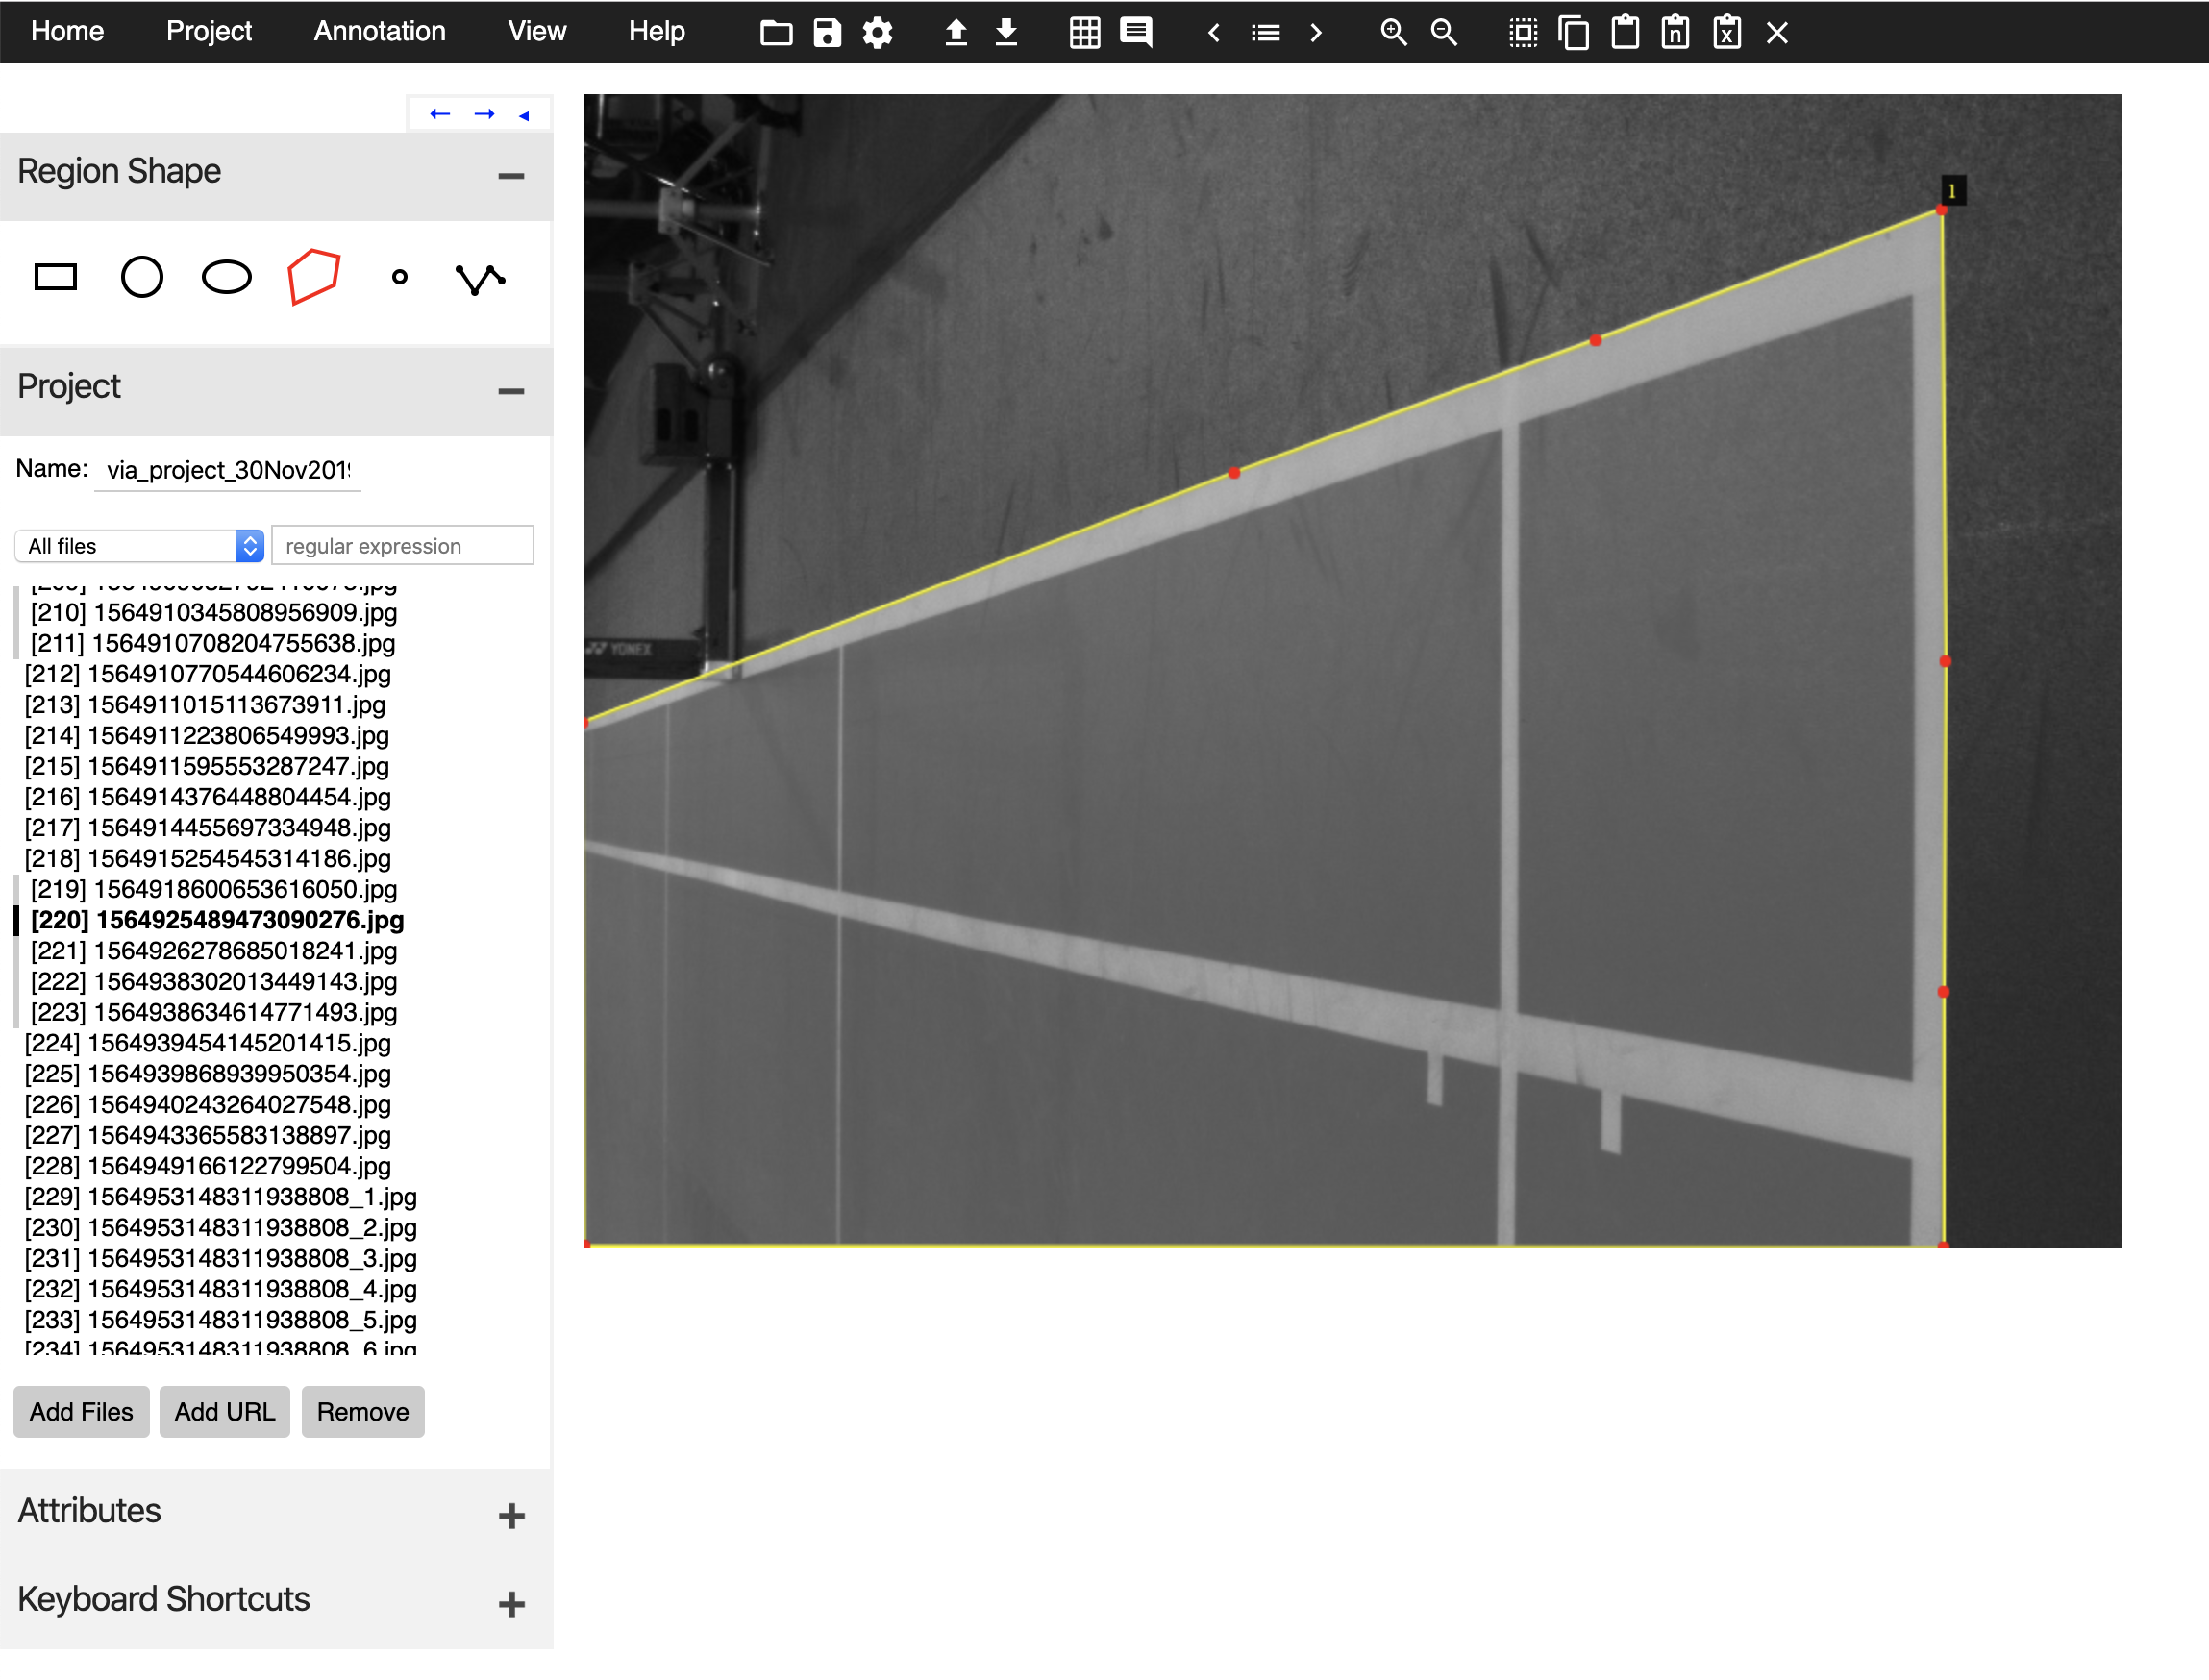
\includegraphics[width=\linewidth]{./via_low.png}
    \caption{Zrzut ekranu uruchomionego anotatora danych na zbiorze \textit{low}}
    \label{fig:vialow}
\end{figure}
